
\chapter{Spannkraftinduzierten Deformation}

Im folgenden Kapitel wird die Methode zur Erkennung und Analyse von durch 
Spannkraft induzierter Deformationen beschrieben. Ziel ist es, 
aus zwei zusammengefügten Bilder von zwei verschiedenen Spannungsstufen, 
Deformationen zu erkennen.
Als Deformation wird eine äußerliche Veränderung des betrachteten Bauteils bezeichnet, 
die äußere Veränderung ist hierbei über den Unterschied der Ränder der Bauteile definiert.
Bevor eine Deformation erkannt werden kann, muss die Randgeometrie von beiden
abgebildeten Bauteilen erfasst werden.
Vorerst werden in einem Schritt immer nur zwei Spannungsstufen miteinander verglichen 
und die Deformationsdaten anschließend abgespeichert.
Die Auswertung der resultierenden Daten erfolgt in einem separaten Schritt, so können auch
mehrere Spannungsstufen untereinander verglichen werden, ohne das die Komplexität steigt.

\section{Deformation zwischen zwei Spannungszuständen}

Wie beschrieben, ist die Deformation zwischen zwei Bauteilen als Differenz der 
Randgeometrie deformiert. Um die Randgeometrie eines Bauteils zu ermitteln, 
kann erneut die Kontursuche [VERWEIS] angewendet werden. Die gefundenen Konturen bilden dann 
die Ränder des Bauteils ab. So werden äußere aber auch innere Geometrien 
abgebildet und ermöglichen die Deformationserkennung. 
In Abbildung \ref{fig:stichted_contour} ist ein 
zusammengefügtes Bild und die erkannte Randgeometrie eines Bauteils zu sehen.

\begin{figure}[H]
    \centering
    \begin{minipage}{0.49\textwidth}
        \centering
        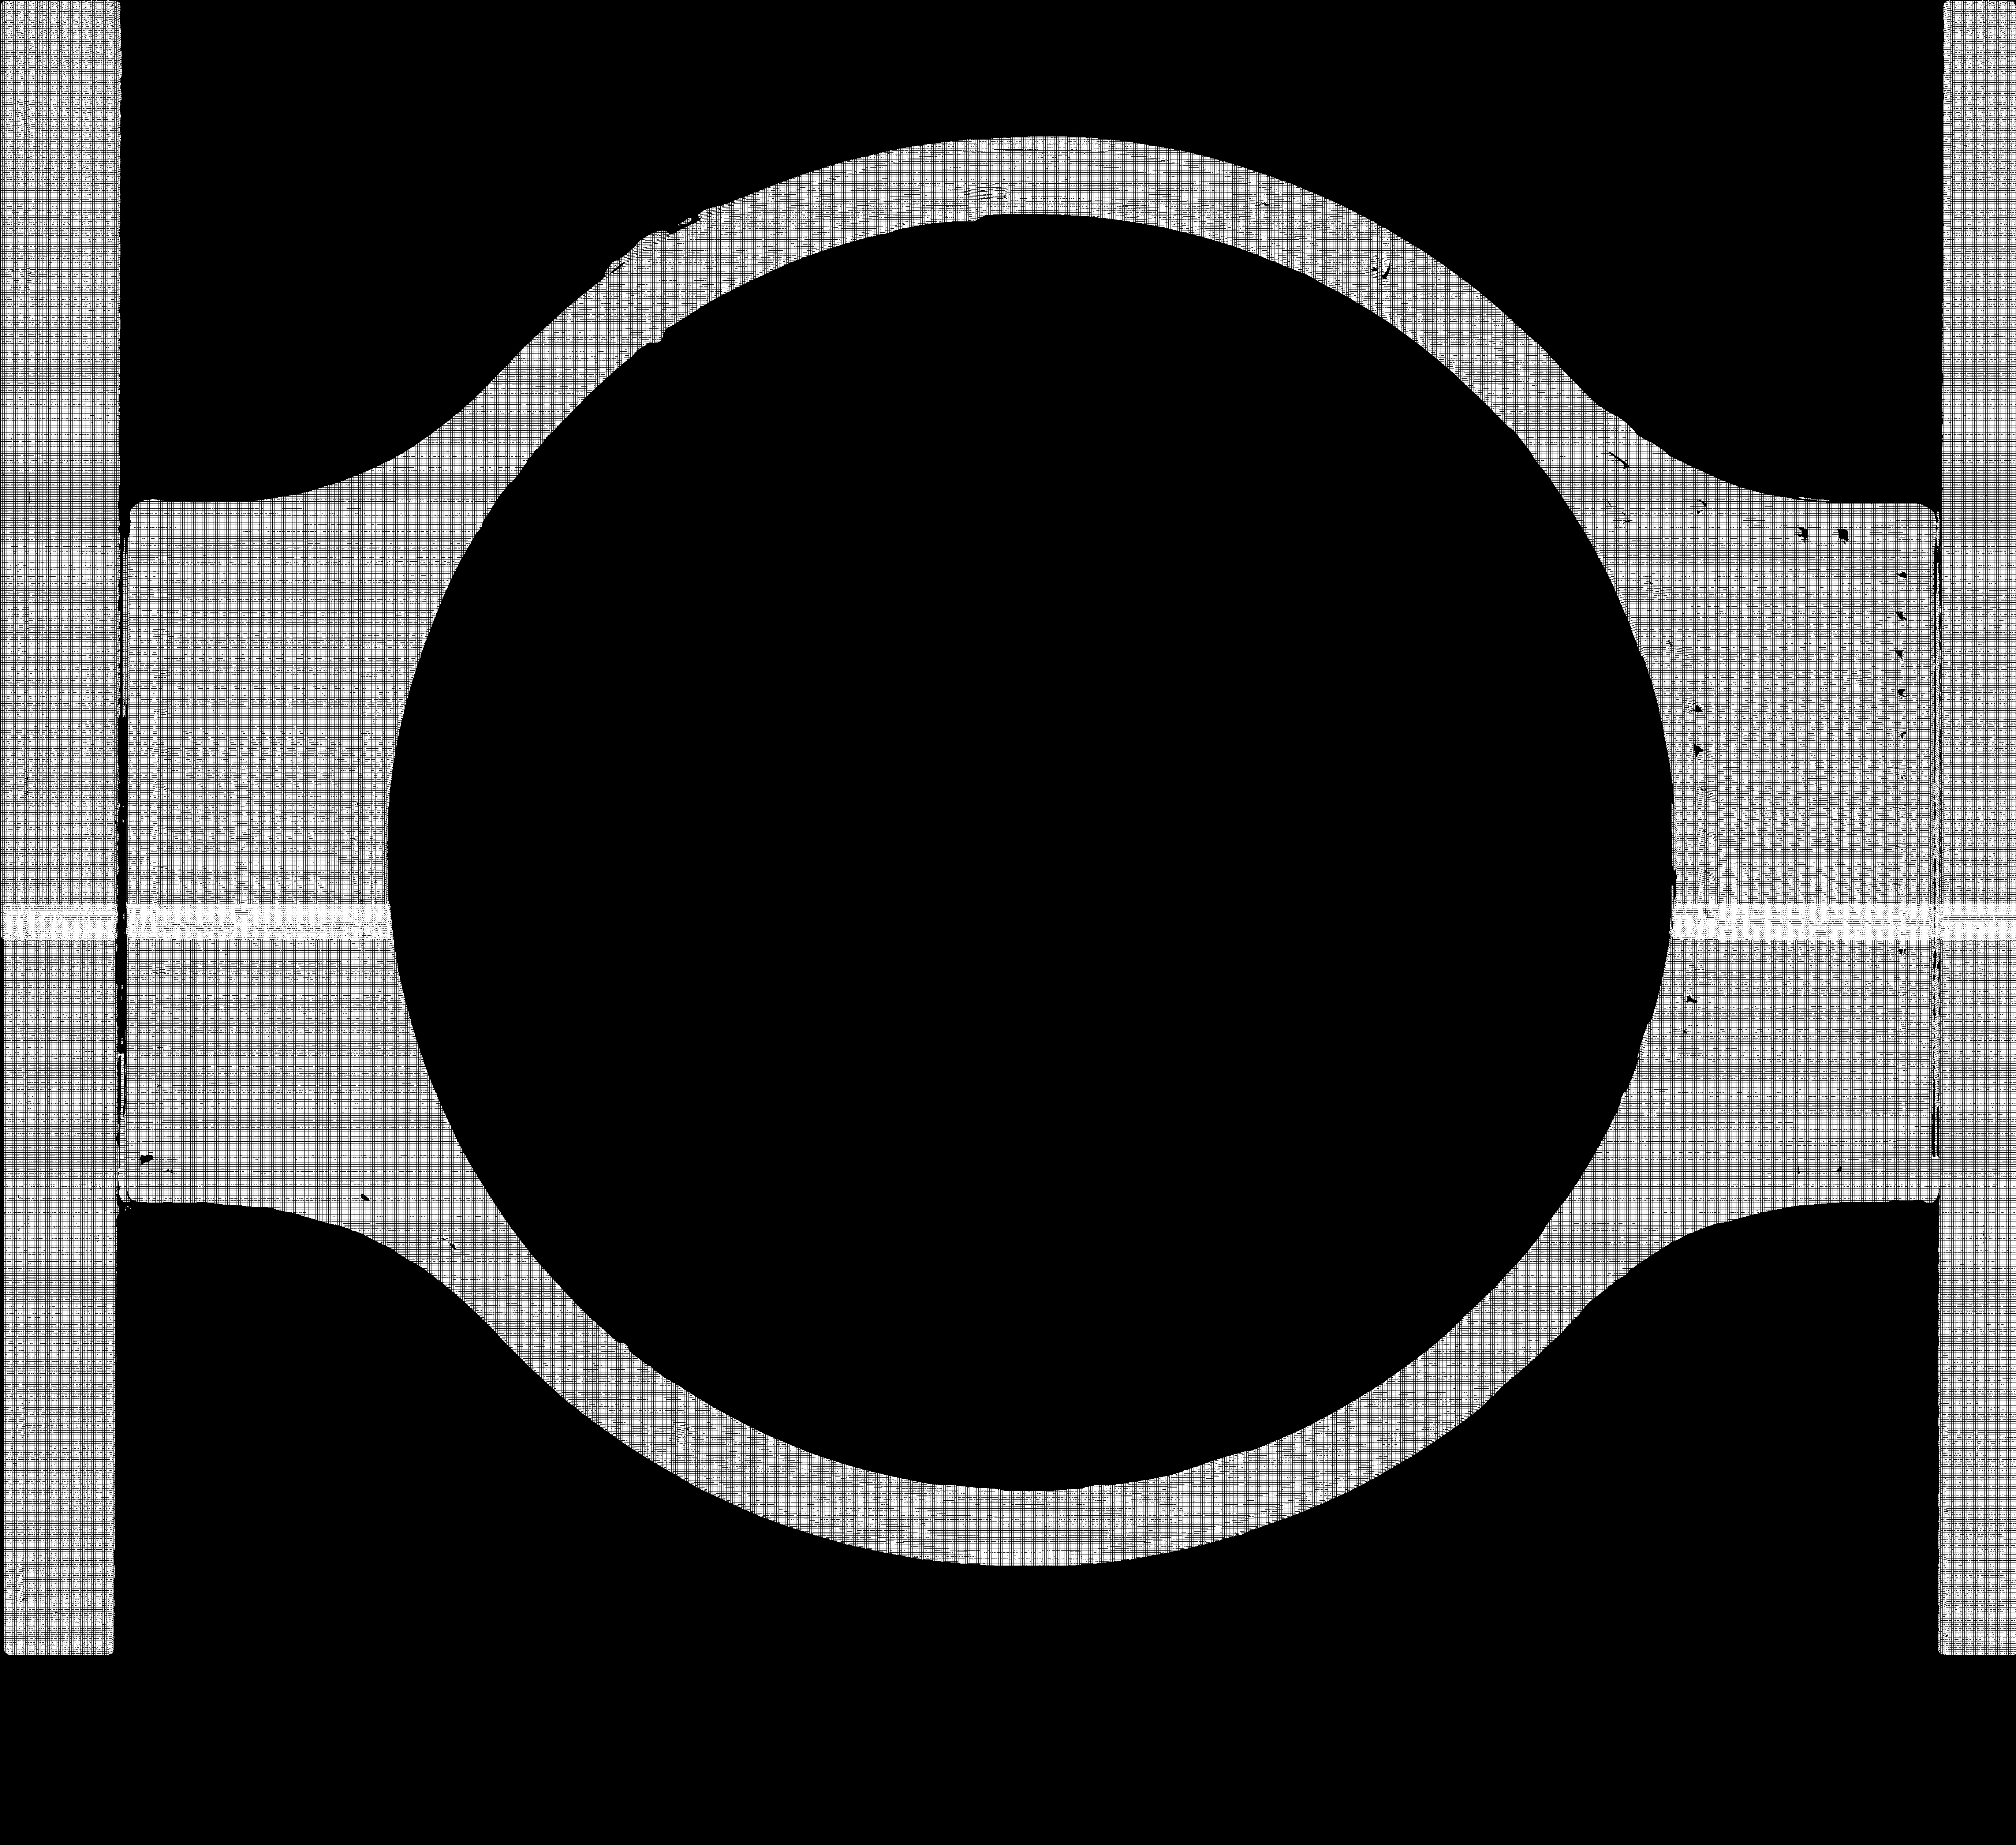
\includegraphics[width=\textwidth]{images/FDM_sp0_stitched.jpg} % first figure itself
        \caption*{(a)} 
    \end{minipage}\hfill
    \begin{minipage}{0.49\textwidth}
        \centering
        \includegraphics[width=\textwidth]{images/contours_FDM_sp0_stitched.jpg} % first figure itself
        \caption*{(b)}
    \end{minipage}\hfill
    \caption{(a) Zusammengefügtes Bild des FDM Demonstratorbauteils, Spannungsstufe 0
    (b) Randgeometrie von (a), die zur Erkennung der Deformation genutzt wird}
        \label{fig:stichted_contour}
\end{figure}

\subsection{Randgeometrien übereinander legen}

Um die Differenz zweier Randgeometrien bilden zu können, müssen diese übereinander 
gelegt werden.
Dies garantiert, dass die gebildete Differenz minimal ist.
Der schon beschriebe Ansatz des Konturmatching [VERWEIS] könnte auch hier genutzt worden. 
allerdings müssen hier die gesamten Konturen betrachtet werden und nicht wie zuvor nur 
der überlappende Auschnitt. Das schon vorgestellte Verfahren ist für die Konturen eines
gesamten Bauteils nicht performant genug um eine akzeptable Laufzeit für das Verfahren
zu gewährleisten. 
Deswegen wird hier ein anderes Verfahren eingesetzt. Es basiert auf demselben Prinzip,
Punktepaare zu finden deren euklidischen Distanz gleich null ist. Anstatt das aber 
jeder Punkt der Zielkontur mit jedem Punkt der Ursprungskontur verglichen wird, 
wird ein maximaler Radius definiert in dem nach benachbarten Punkten gesucht wird.
Hierfür muss die Kontur erst in eine zweidimensionale Datenstruktur überführt werden.
Dieser zusätzliche Aufwand sorgt für eine deutlich verkürzte Laufzeit.

Ähnlich zu dem schon beschriebenen ICP-Algorithmus [VERWEIS] wird eine Transformation berechnet,
mit der eine Kontur einer anderen Kontur angenähert werden kann.
Die Transformation wird mit folgendem Algorithmus berechnet:
(FRAGE: Hier entweder das, oder latex-pseudocodeblock, oder python screenshot?).

\begin{enumerate}
    \item Zu jedem Punkt in der Ursprungskontur wird der Nachbarpunkt
    in der Zielkontur gesucht, der den kleinsten euklidischen Abstand besitzt.
    \item Wird kein solcher Punkt in einem definierten Radius gefunden,
    wird der nächste Punkt der Ursprungskontur
    betrachtet. Falls ein Punkt gefunden wurde, wird der Vektor gebildet der die Punkte
    der Ursprungs- und Zielkontur verbindet.
    \item Wenn alle Punkte der Ursprungskontur betrachtet sind, wird der 
    Durchschnitt aller gefunden Vektoren gebildet.
    \item Da die Transformation auf Pixel angewendet wird, muss sie ganzen Zahlen 
    entsprechen. Wenn der Absolutwert beider Vektorelemente der Transformation 
    unter 0.2 Pixel fällt wird die Transformation auf (0, 0) gerundet.
    Ansonsten wird auf die nächste ganze Zahl gerundet.
\end{enumerate}

Ist die Transformation ungleich dem Vektor (0, 0) wird sie auf die Ursprungskontur 
angewendet und erneut die Transformation berechnet. Dies wird so lange wiederholt bis 
die Transformation dem Nullvektor entspricht. Wenn dies geschieht, sind beide Konturen, 
und damit die Randgeometrien der Bauteile angenähert.
Um Rechenzeit zu sparen werden vor dem Ermitteln der ersten Transformation die 
Massenmittelpunkte beider Bauteilgeometrien berechnet und übereinader gelegt.

\subsection{Deformation messen}

[Deformation ausführlich beschreiben]
Nachdem die beschriebenen Schritte erfolgt sind, kann die Deformation bestimmt werden.
Hierfür wird über die gesamte x-Achse des Bildes iteriert und die kleinste Differenz 
zwischen zwei Punkten gebildet. Diese entspricht dann einer Abweichung. 
Da innere und äußere Randgeometrie separat betrachtet werden, kann es immer nur zwei
solcher Punktepaare geben, eins am oberen Ende des Bauteils und eins am unteren Ende.
Es wird der euklidische Abstand beider Punktepaare gebildet und aufsummiert.
So entsteht ein Datensatz für ein Bild, 
dass die Differenz zweier Spannungsstufen ausgibt. In Abbildung \ref{fig:deformation_data}
ist ein solcher Datensatz zu sehen. 

Innere und äußere Randgeometrien werden separat betrachtet und analysiert.
In Abbildung \ref{fig:deformation_data_vis} ist die Deformation des inneren Kreises
visuell dargestellt. In Abbildung \ref{fig:deformation_data_graph} sind die 
Deformationswerte grafisch dargestellt.

Es wurde ein per FDM gefertigtes Bauteil eingespannt und zwei Spannungsstufen verglichen.
Die Blau sehende Linie bildet die Randgeometrie des Bauteils ab, dass mit Spannungsstufe
null eingespannt wurde. Das entspricht hier nur einer lockerer Einspannung bei 

\begin{figure}[H]
    \centering
    \includegraphics[width=0.99\textwidth]{images/FDM2_SP0_stitched_FDM2_SP4_stitched_1_1_cut.png}
    \caption{Deformation der inneren Bauteilgeometrie des Demonstratorbauteils 
    visuell dargestellt}
    \label{fig:deformation_data_vis}
\end{figure}


\begin{figure}[H]
    \centering
    \includegraphics[width=0.9\textwidth]{images/FDM_sp0_sp4_inner.png}
    \caption{Deformation der inneren Bauteilgeometrie 
    des Demonstratorbauteils als Graph}
    \label{fig:deformation_data_graph}
\end{figure}

Es ist gut zu erkennen, dass sich das Bauteil 
im mittleren Bereich ausgedehnt hat und in den Randbereichen schmaler geworden ist.
Dieser Datensatz unterliegt einer relativ großen Streuung. Um mehrere Spannungsstufen
zu vergleichen, wird der Datensatz zu einer Geraden zusammengefasst.
Diese Gerade ist auch in \ref{fig:deformation_data} in Blau zu sehen. Sie wird 
gebildet, indem immer zehn Datenpunkte zu einem zusammengefasst werden. 
So können auch mehrere Spannungsstufen visuell dargestellt und verglichen werden.

\begin{figure}[H]
    \centering
    \includegraphics[width=0.7\textwidth]{images/FDM_sp0_sp3_defo_plot.png}
    \caption{Differenz von zwei Spannungsstufen bei einem FDM Bauteil, äußere 
    Bauteilgeometrie.}
    \label{fig:deformation_data}
\end{figure}

\begin{figure}[H]
    \centering
    \includegraphics[width=0.7\textwidth]{images/FDM_sp0_many_defo_plot2.png}
    \caption{Differenz von mehreren Spannungsstufen bei einem FDM Bauteil}
    \label{fig:deformation_data_all}
\end{figure}



